%%%%%%%%%%%%%%%%%%%%%%%%%%%%%%%%%%%%%%%%%%%%%%%%%%%%%%%%%%%%%%%%%%%%%%%%%%%%%%%%%%%%
% Document data
%%%%%%%%%%%%%%%%%%%%%%%%%%%%%%%%%%%%%%%%%%%%%%%%%%%%%%%%%%%%%%%%%%%%%%%%%%%%%%%%%%%%
\documentclass[12pt]{article} %report allows for chapters
%%%%%%%%%%%%%%%%%%%%%%%%%%%%%%%%%%%%%%%%%%%%%%%%%%%%%%%%%%%%%%%%%%%%%%%%%%%%%%%%%%%%
\usepackage{preamble}

\begin{document}

\begin{center}
   \textsc{\large MATH 271, Homework 9, \emph{Solutions}}\\
   \textsc{Due November 15$^\textrm{th}$}
\end{center}
\vspace{.5cm}



\begin{problem}
Compute the following:
\begin{enumerate}[(a)]
    \item 
    \[
    [A]=\begin{pmatrix} 1& 1& 1 \end{pmatrix}
    \begin{pmatrix} 2\\ 1\\ 3 \end{pmatrix}.
    \]
    \item
    \[
    [B]=\begin{pmatrix} 1& 2& 3& 4\\ 5& 6& 7& 8\\ 9& 10& 11& 12\end{pmatrix}
    \begin{pmatrix} 3& 2\\ 2& 3\\ 3& 2\\ 2& 3\end{pmatrix}
    \]
    \item Take
    \[
    [M]=\begin{pmatrix} 10& 15\\ 20& 10 \end{pmatrix}
    \]
    and
    \[
    [N]=\begin{pmatrix} 1 & 2\\ 2& 1\end{pmatrix}.
    \]
    Compute $[M][N]$ and $[N][M]$ to see that matrices do not commute in general.
\end{enumerate}
\end{problem}
\begin{solution}~
\begin{enumerate}[(a)]
    \item Since we have a $1\times 3$-matrix multiplied with a $3\times 1$-matrix, we know that $[A]$ should be a $1\times 1$-matrix.
    \begin{align*}
    [A]&=\begin{pmatrix} 1 & 1 & 1 \end{pmatrix} \begin{pmatrix} 2 \\ 1 \\ 3 \end{pmatrix}\\
    &= (1\cdot 2 + 1 \cdot 1 + 1 \cdot 3)\\
    &= (6).
    \end{align*}
    \item Here, we should expect that $[B]$ is a $3\times 2$-matrix.
    \[
    [B] = \begin{pmatrix} 24 & 26 \\ 64 & 66 \\ 104 & 106 \end{pmatrix}.
    \]
    \item Here $[M]$ and $[N]$ are square, so multiplying will give us the same shape matrix.  We have
    \[
    [M][N] = \begin{pmatrix} 40 & 35 \\ 40 & 50 \end{pmatrix},
    \]
    as well as
    \[
    [N][M] = \begin{pmatrix} 50 & 35 \\ 40 & 40 \end{pmatrix}.
    \]
    From this we can see that $[M][N]\neq [N][M]$ in general!
\end{enumerate}
\end{solution}

\newpage
\begin{problem}
A linear transformation $T\colon \R^3 \to \R^3$ is given by the matrix
\[
[T]= \begin{pmatrix}
1& 2& 0\\
2& 1& 2\\
0& 2& 1
\end{pmatrix}.
\]
\begin{enumerate}[(a)]
    \item Compute how $T$ transforms the standard basis elements for $\R^3$. That is, find
    \[
    T(\xhat), \qquad
    T(\yhat), \qquad 
    T(\zhat).
    \]
    This gives a nice interpretation of matrix vector multiplication as linear combinations of the column vectors that make up a matrix.
    \item If we apply this linear transformation to the unit cube (that is, all points who have $(x,y,z)$ coordinates with $0\leq x \leq 1$, $0\leq y \leq 1$, and $0\leq z \leq 1$), what will the volume of the transformed cube be? (\emph{Hint: the determinant of this matrix $[T]$ provides us this information.})
\end{enumerate}
\end{problem}
\begin{solution}~
\begin{enumerate}[(a)]
    \item The point here is that we can understand the matrix $[T]$ and matrix multiplication better by seeing how the basis vectors are transformed. So we have
    \begin{align*}
        T(\xhat) &= \begin{pmatrix}
1& 2& 0\\
2& 1& 2\\
0& 2& 1
\end{pmatrix} \begin{pmatrix} 1 \\ 0 \\ 0 \end{pmatrix}\\
&= \begin{pmatrix} 1 \\ 2 \\ 0 \end{pmatrix},
    \end{align*}
    which is just the first column of the matrix. Then we have
    \begin{align*}
                T(\yhat) &= \begin{pmatrix}
1& 2& 0\\
2& 1& 2\\
0& 2& 1
\end{pmatrix} \begin{pmatrix} 0 \\ 1 \\ 0 \end{pmatrix}\\
&= \begin{pmatrix} 2 \\ 1 \\ 2 \end{pmatrix},
    \end{align*}
    which is just the second column of the matrix. Lastly we have
    \begin{align*}
                T(\zhat) &= \begin{pmatrix}
1& 2& 0\\
2& 1& 2\\
0& 2& 1
\end{pmatrix} \begin{pmatrix} 0 \\ 0 \\ 1 \end{pmatrix}\\
&= \begin{pmatrix} 0 \\ 2 \\ 1 \end{pmatrix},
    \end{align*}
    which is the last column of the matrix.
    \item The three basis vectors 
    \[
    \xhat = \begin{pmatrix} 1 \\ 0 \\ 0 \end{pmatrix}, \qquad \yhat = \begin{pmatrix} 0 \\ 1 \\ 0 \end{pmatrix}, \qquad \zhat =\begin{pmatrix} 0 \\ 0 \\ 1 \end{pmatrix}
    \]
    define the volume of the unit cube. That is, the parallelepiped generated by $\xhat$, $\yhat$, and $\zhat$ is the unit cube. Hence, if we know how these vectors are transformed, we just need to find the volume of the paralellepiped given by the transformed vectors $T(\xhat)$, $T(\yhat)$, and $T(\zhat)$.  Now, we can collect these vectors into a matrix,
    \begin{align*}
    \begin{pmatrix} \vert & \vert & \vert \\ T(\xhat) & T(\yhat) & T(\zhat) \\ \vert & \vert & \vert \end{pmatrix} &= \begin{pmatrix}  1& 2& 0\\
2& 1& 2\\
0& 2& 1\end{pmatrix},
    \end{align*}
    which is exactly $[T]$! This is what we realized in part (a)! Now, the determinant of the matrix gives us the signed volume of the parallelepiped generated by the three column vectors, and hence
    \[
    \mathrm{Area}=|\det([T])|=|-7|=7.
    \]
\end{enumerate}
\end{solution}

\newpage
\begin{problem}
Consider some linear transformation $T\colon \R^n \to \R^m$.  Let $\vecv_1, \dots, \vecv_k$ be vectors in $\operatorname{Null}(T)$.  
\begin{enumerate}[(a)]
    \item Show that the span of these vectors is also in the nullspace of $T$.
    \item How many linearly independent vectors can be in the nullspace?
\end{enumerate}
\end{problem}
\begin{solution} In this problem one can see that the nullspace for a linear transformation $T$ is invariant.  What I mean is that if we take linear combinations of vectors in the nullspace, they remain in the nullspace.  Fundamentally, this comes down to something a bit more general as the nullspace is a special case of an eigenspace. See Worksheet 9 Problem 4 for example or Chapter 9 \S 8..  

Then, we consider the ``best" and ``worst" cases for the nullspace based on the dimensions involved in the transformation.  That is, the input dimension $n$ and the output dimension $m$ completely dictate how many vectors can at most and at least be in the nullspace for $T$.

\begin{enumerate}[(a)]
    \item An arbitrary vector $\vecv$ in the span of $\vecv_1,\dots,\vecv_k$ is given by
    \[
    \vecv= \alpha_1 \vecv_1 + \alpha_2 \vecv 2 + \cdots + \alpha_k \vecv_k.
    \]
    Since $\vecv$ is arbitrary, if we show $\vecv \in \operatorname{Null}(T)$, then we are done.  So we take
    \begin{align*}
        T(\vecv) &= T(\alpha_1 \vecv_1 + \alpha_2 \vecv_2 + \cdots + \alpha_k \vecv_k )\\
        &= \alpha_1 T(\vecv_1) + \alpha_2 T(\vecv_2) + \cdots + \alpha_k T(\vecv_k) && \textrm{by linearity of $T$}\\
        &= 0 &&\textrm{since $T(\vecv_i)=0$ for all $i=1,\dots, k$.}
    \end{align*}
    Thus the span of $\vecv_1,\dots,\vecv_k$ is also in the nullspace of $T$.
    \item With $T\colon \R^n \to \R^m$ we can take the transformation $T(\vecv)=\zerovec$ for every vector $\vecv \in \R^n$.  Note that this transformation always exists and will always have the largest nullspace.  Thus, the nullspace of $T$ would have as many as $n$-linearly independent vectors since there can be at most $n$-linearly independent vectors in $\R^n$. This fact is independent of the value for $m$.

    Taking $m$ into account now, if $m<n$, then we must have $n-m$ vectors in the nullspace of $T$ at the very least. The argument is somewhat geometrical as $T$ removes $n-m$ dimensions in the process and as such, we remove $n-m$ linearly independent vectors (as those vectors span those removed dimensions).  Thus, if $m<n$ we have that
    \[
        n-m \leq \textrm{number of L.I. vectors in nullspace of $T$} \leq n.
    \]
    In the case $m\geq n$ we have
    \[
       0 \leq \textrm{number of L.I. vectors in nullspace of $T$} \leq n.
    \]
    To see why this is true, we let $\vecv = v_1 \xhat_1 + v_2 \xhat_2 + \cdots + v_n \xhat _n$ and note that if $m\geq n$ we can take 
    \[
    T(\vecv) = v_1 \xhat_1 + v_2 \xhat_2 + \cdots + v_n \xhat_n + 0 \xhat_{n+1} +\cdots + 0 \xhat_{m},
    \]
    which shows that there are no nontrivial vectors in the nullspace of this $T$.  
    
\end{enumerate} 

\end{solution}


\newpage
\begin{problem}~
\begin{enumerate}[(a)]
    \item Show that for any $2\times 2$-matrix that the sign of the determinant changes if either a row or column is swapped. \emph{Note: this is true for square matrices of any size}.
    \item Show that for any $2\times 2$-matrix that multiplying a column by a constant scales the determinant by that constant as well. \emph{Note: this is true for square matrices of any size.}
    \item Show that for any $2\times 2$-matrix that adding a scalar multiple one column to the other will not change the determinant. \emph{Note: this is true in broader generality. In fact, adding linear combinations of columns to another column will not change the determinant.}
    \item Using these facts, argue that a square matrix with columns that are linearly dependent must have a determinant of zero.
\end{enumerate}
\end{problem}
\begin{solution}~
\begin{enumerate}[(a)]
    \item Let
    \[
    [A]=\begin{pmatrix} a & b \\ c & d \end{pmatrix}
    \]
    be an arbitrary $2\times 2$-matrix.  Then we have
    \[
    \det([A])=ad-bc.
    \]
    Now, if we swap rows we have
    \[
    \left| \begin{matrix} c & d \\ a & b \end{matrix} \right| = bc-ad = -(ad-bc).
    \]
    Now, we can do the same with columns to get
    \[
    \left| \begin{matrix} b & a \\ d & c \end{matrix} \right| = bc-ad = -(ad-bc).
    \]
    \item Let us compute the determinant of
    \[
    \left| \begin{matrix} \alpha a & b \\ \alpha c & d \end{matrix} \right| = \alpha ad - \alpha bc = \alpha(ad-bc).
    \]
    Similarly, we will have the same if we scale the other column. In fact, this is true for rows as well.
    \item Let us add the first column to the second. We get
    \[
     \left| \begin{matrix} \alpha a & \alpha a+b \\ \alpha c & \alpha c+d \end{matrix} \right| = a(\alpha c+d)-(\alpha a+b)c = \alpha ac+ad-\alpha ac-bc = ad-bc.
    \]
    The same will be true if we add a scalar copy of column 2 to column 1.
    \item Let us just show this for a $3\times 3$-matrix as the argument is the same for the most general case.  Let 
\[
[A] = \begin{pmatrix} \vert & \vert & \vert \\ \colA_1 & \colA_2 & \colA_3 \\ \vert & \vert & \vert \end{pmatrix}.
\]
Then if the columns of $[A]$ are linearly dependent, we have that
\[
\alpha_1 \colA_1 + \alpha_2 \colA_2 + \alpha_3 \colA_3 = \zerovec
\]
with at least one $\alpha_i\neq 0$.  Specifically, this means that one vector can be written as a linear combination of the others. That is we can take
\[
\colA_3 = \frac{-1}{\alpha_3} (\alpha_1 \colA_1 + \alpha_2 \colA_2),
\]
so long as $\alpha_3\neq 0$.  If $\alpha_3 = 0$, then choose another vector to write as a linear combination of the others. Then, we can subtract the quantity 
\[
\frac{-1}{\alpha_3} (\alpha_1 \colA_1 + \alpha_2 \colA_2)
\]
from column 3 in $[A]$ to get
\[
\begin{pmatrix} \vert & \vert & \vert \\ \colA_1 & \colA_2 & \zerovec \\ \vert & \vert & \vert \end{pmatrix},
\]
which has a determinant of zero. Since we only added a linear combination of columns to another column, this did not change the determinant and hence we must have $\det([A])=0$.
\end{enumerate}
\end{solution}

\newpage
\begin{problem}
Consider the equation
\[
[A]\vecv = \zerovec,
\]
where
\[
[A] = \begin{pmatrix} 0 & 1 & 0 \\ 1 & 0 & 1 \\ 0 & 1 & 0 \end{pmatrix}.
\]
\begin{enumerate}[(a)]
    \item Are the columns of $[A]$ linearly independent or dependent? Explain.
    \item What vector(s) $\vecv$ satisfy this equation? In other words, what is $\Null([A])$?
    \item Using what you found above, what must $\det([A])$ be equal to? \emph{Hint: you do not need to compute the determinant!}
\end{enumerate}
\end{problem}
\begin{solution}~
\begin{enumerate}[(a)]
    \item The columns are dependent as the leftmost column is equal to the rightmost column.
    \item To solve the homogeneous equation we take
    \begin{align*}
        [M]=\left(\begin{array}{ccc|c}
            0 & 1 & 0 &0 \\
            1 & 0 & 1 &0\\
            0 & 1 & 0 &0
        \end{array}\right).
    \end{align*}
    Then we can subtract row one from row three to get
    \[
    \left(\begin{array}{ccc|c}
            0 & 1 & 0 &0\\
            1 & 0 & 1 &0\\
            0 & 0 & 0 &0
        \end{array}\right)
    \]
    which corresponds to the equations
    \begin{align*}
        0x+y+0z&=0\\
        x+0y+z&=0\\
        0x+0y+0z&=0.
    \end{align*}
    Hence we have that $z=-x$ and $y=0$.  Thus any vector of the form
    \[
    \vecv = \begin{pmatrix} t \\ 0 \\ -t \end{pmatrix}
    \]
    for any $t\in \R$ is a solution to this equation. In other words, the set described above is $\Null([A])$.
    \item The determinant must be equal to zero since $\Null([A])$ is nontrivial (i.e., it contains more than just the zero vector). One can also note the columns are dependent which implies this as well.  This goes to show a bit on how these ideas are all connected.
\end{enumerate}
\end{solution}

\newpage
\begin{problem}
Compute the following determinants:
\begin{enumerate}[(a)]
    \item
    \[
    \det([A])=\left| \begin{array}{ccc}
    -3& 1 & 5\\
    -3& 4 & 2\\
    -3& 2 & 1
    \end{array}\right|
    \]
    \item 
    \[
    \det([B])=\left| \begin{array}{ccc}
    1& 2& 3\\
    4& 5& 6\\
    7& 8& 9
    \end{array}\right|
    \]
    \item Compute $\det([A][B])$ using properties of the determinant. \emph{Hint: this should be very quick to do. Do not compute the product of the matrices $[A]$ and $[B]$!}
\end{enumerate}
\end{problem}
\begin{solution}~
\begin{enumerate}[(a)]
    \item We can expand along any row or column and in this case, there are no zeros to make the computation quicker. So we have
    \begin{align*}
        \left| \begin{matrix} -3 & 1 & 5 \\ -3 & 4 & 2 \\ -3 & 2 & 1 \end{matrix} \right| &= -3 \left| \begin{matrix} 4 & 2 \\ 2 & 1 \end{matrix} \right| -1 \left| \begin{matrix} -3 & 2 \\ -3 & 1 \end{matrix} \right| +5 \left| \begin{matrix} -3 & 4 \\ -3 & 2 \end{matrix} \right|\\
        &= -3(4-4)-1(-3+6)+5(-6+12)\\
        &= 27.
    \end{align*}
    \item Similarly, we get
    \[
    \det([B])= 0.
    \]
    \item We know that $\det([A][B])=\det([A])\det([B])$ and thus we have that $\det([A][B])=0.$
\end{enumerate}
\end{solution}


\newpage
\begin{problem}~
\begin{enumerate}[(a)]
    \item What does a zero determinant indicate about the solutions of a non-homogeneous system of linear equations? (Think geometrically!)
    \item What does a zero determinant indicate about the solutions of a homogeneous system of linear equatoins? (Think geometrically!)
\end{enumerate}
\end{problem}
\begin{solution}~
\begin{enumerate}[(a)]

    \item If the determinant of a matrix is zero, that means the span of the columns is not the whole entire vector space.  Take for example the matrix,
\[
[A]=\begin{pmatrix} 1 & 0 & 0 \\ 0 & 1 & 0 \\ 0 & 0 & 0 \end{pmatrix}.
\]
More explanation for the transformation given by this matrix is found in Chapter 9 \S 6 of the text. I'll copy the visualization over.
        \begin{figure}[H]
            \centering
            \resizebox{.6\textwidth}{!}{\input{linear_transform_kernel.pdf_tex}}
            %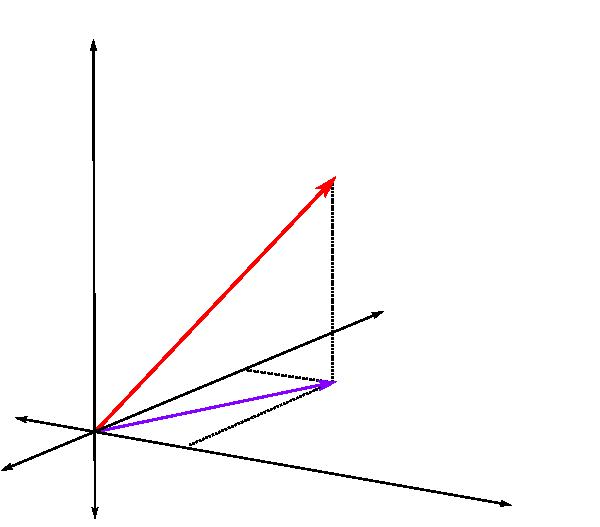
\includegraphics[width=.7\textwidth]{Figures_Part_4/linear_transform_kernel.pdf_tex}
        \end{figure}
Notice that this transformation finds the ``shadow" of the vector in the $xy$-plane. One can note now that columns of this matrix only span the $xy$-plane and this is realized geometrically as for any vector $\vecv$, $[A]\vecv$ will only have a zero $z$-component. For example,
\[
\begin{pmatrix} 1 & 0 & 0 \\ 0 & 1 & 0 \\ 0 & 0 & 0 \end{pmatrix} \begin{pmatrix} x \\ y \\ z \end{pmatrix} = \begin{pmatrix} x \\ y \\ 0 \end{pmatrix}.
\]
Hence, for sake of example, if I take the inhomogeneous equation
\[
\begin{pmatrix} 1 & 0 & 0 \\ 0 & 1 & 0 \\ 0 & 0 & 0 \end{pmatrix} \begin{pmatrix} x \\ y \\ z \end{pmatrix} = \begin{pmatrix} 0 \\ 0 \\ 1 \end{pmatrix}
\]
we get the equation
\[
x\xhat + y\yhat = \zhat,
\]
which has no solution! Geometrically, this is due to the fact that the span of the columns of $[A]$ doesn't contain the vector $\zhat$. Hence, a zero determinant means we cannot necessarily solve non-homogeneous equations.  If we instead had the equation
\[
\begin{pmatrix} 1 & 0 & 0 \\ 0 & 1 & 0 \\ 0 & 0 & 0 \end{pmatrix} \begin{pmatrix} x \\ y \\ z \end{pmatrix} = \begin{pmatrix} 1 \\ 1 \\ 0 \end{pmatrix},
\]
then this gives us the equation
\[
x\xhat + y\yhat = \xhat + \yhat,
\]
which means we must have $x=1$ and $y=1$. However, $z$ is free to be anything, which means any vector of the form
\[
\begin{pmatrix} 1 \\ 1 \\ z\end{pmatrix},
\]
is a solution! But, this is not a unique solution. 

    \item A zero determinant for a matrix $[A]$ is equivalent to the fact that the columns are linearly dependent. Thus, this means some of the vectors are redundant. If $[A]$ is an $n\times n$-matrix, then the columns of $[A]$ could span at most $n-1$ dimensions and there must be at least one direction that is transformed to zero under the matrix $[A]$.

    Take my example from the previous problem.  There the columns only spanned the $xy$-plane and thus the $z$-direction is squished to zero by that matrix.  So there were infinitely many solutions to the homogeneous equation. More explicitly, take a vector $\vecv = z\zhat$, then
    \[
    [A]\vecv = \begin{pmatrix} 1 & 0 & 0 \\ 0 & 1 & 0 \\ 0 & 0 & 0 \end{pmatrix} \begin{pmatrix} 0 \\ 0 \\ z \end{pmatrix} = \begin{pmatrix} 0 \\ 0 \\ 0 \end{pmatrix}.
    \]
    Geometrically, this is saying that the nullspace of $[A]$ is spanned by the vector $\zhat$ and so any scalar copy of $\zhat$ is also in the nullspace. One can picture this as having the transformation take the whole $z$-axis and squish it down to a length of zero.
\end{enumerate}
\end{solution}

\newpage
\begin{problem}
Given the matrices
\[
[A]=\begin{pmatrix} 1 & 0 & 2 \\ 2  & 1 & 3 \\ -2 & -2 & 0 \end{pmatrix} \qquad \textrm{and} \qquad [B]=\begin{pmatrix} -3 & 1 & 1 \\ 2 & -2 & 4 \\ -1 & -1 & -1 \end{pmatrix}.
\]
\begin{enumerate}[(a)]
    \item Compute $\tr([A])$ and $\tr([B])$.  
    \item Compute $\tr([A][B])$ and compare it to $\tr([B][A])$.
\end{enumerate}
\end{problem}
\begin{solution}~
\begin{enumerate}[(a)]
    \item The traec is the sum of the diagonal entries. Thus we have
    \begin{align*}
        \tr([A])&=1+1+0=2,\\
        \tr([B])&=-3-2-1=-6.
    \end{align*}
    \item Then we can compute $[A][B]$,
    \[
    [A][B]=\begin{pmatrix}
    -5 & -1 & -1 \\ -7 & -3 & 3 \\ 2 & 2 & -10
    \end{pmatrix}.
    \]
    Hence we have
    \[
    \tr([A][B]) = -18.
    \]
    Note that under cyclic permutations, the trace is invariant, hence
    \[
    \tr([A][B])=\tr([B][A])
    \]
    even though $[A][B]\neq [B][A]$
    
\end{enumerate}
\end{solution}


\end{document}